\documentclass{beamer}[10]

\usepackage{graphicx}
\usepackage{xcolor}
\usepackage{tabto}
%\usepackage{beamerthemesplit}
\usepackage{tikz}
\usepackage{cancel}
\usepackage{verbatim}
\usepackage{fancybox}
\usepackage{enumerate}
\usepackage{amsmath,amssymb,amsthm,textcomp,mathtools}
\usepackage[super]{nth}
\usepackage[amssymb]{SIunits}
\usepackage{booktabs}
\usepackage{cancel}
\usepackage{bm}
\usepackage[utf8]{inputenc}
\usepackage{tabularx}
\usepackage{ragged2e}
\newcolumntype{Y}{ >{\RaggedRight\arraybackslash}X}
\usetikzlibrary{arrows,shapes}
\newcommand\T{\rule{0pt}{2.6ex}}
\newcommand\B{\rule[-1.2ex]{0pt}{0pt}}
\definecolor{UUcrimson}{RGB}{204,0,0}
\mode<presentation>
{ \usetheme{default}
  \usecolortheme[named=UUcrimson]{structure}
  \useinnertheme{circles}
  \setbeamercovered{transparent}
  \setbeamertemplate{blocks}[rounded]
  \usefonttheme[onlymath]{serif}
  \setbeamertemplate{navigation symbols}{}
  \setbeamertemplate{footline}[page number]
  \setbeamertemplate{navigation symbols}{}
  \setbeamercolor{section in toc}{fg=black,bg=white}
  \setbeamercolor{alerted text}{fg=UUcrimson!80!gray}
  \setbeamercolor*{palette primary}{fg=white,bg=UUcrimson}
  \setbeamercolor*{palette secondary}{fg=UUcrimson!70!black,bg=gray!15!white}
  \setbeamercolor*{palette tertiary}{bg=UUcrimson!80!black,fg=gray!10!white}
  \setbeamercolor*{palette quaternary}{fg=UUcrimson,bg=gray!5!white}
  \setbeamercolor*{palette sidebar primary}{fg=UUcrimson!10!black}
  \setbeamercolor*{palette sidebar secondary}{fg=white}
  \setbeamercolor*{palette sidebar tertiary}{fg=UUcrimson!50!black}
  \setbeamercolor*{palette sidebar quaternary}{fg=gray!10!white}
  \setbeamercolor{titlelike}{parent=palette primary,fg=white}
  \setbeamercolor{frametitle}{bg=UUcrimson}
  \setbeamercolor{frametitle right}{bg=UUcrimson}
  \setbeamercolor*{separation line}{}
  \setbeamercolor*{fine separation line}{}
}

\usetikzlibrary{backgrounds}
\makeatletter
\tikzstyle{every picture}+=[remember picture]
\tikzset{%
  fancy quotes/.style={
    text width=\fq@width pt,
    align=justify,
    inner sep=1em,
    anchor=north west,
    minimum width=\linewidth,
    font=\itshape
  },
  fancy quotes width/.initial={.8\linewidth},
  fancy quotes marks/.style={
    scale=8,
    text=white,
    inner sep=0pt,
  },
  fancy quotes opening/.style={
    fancy quotes marks,
  },
  fancy quotes closing/.style={
    fancy quotes marks,
  },
  fancy quotes background/.style={
    show background rectangle,
    inner frame xsep=0pt,
    background rectangle/.style={
      fill=gray!25,
      rounded corners,
    },
  }
}
\newenvironment{fancyquotes}[1][]{%
\noindent
\tikzpicture[fancy quotes background]
\node[fancy quotes opening,anchor=north west] (fq@ul) at (0,0) {``};
\tikz@scan@one@point\pgfutil@firstofone(fq@ul.east)
\pgfmathsetmacro{\fq@width}{\linewidth - 2*\pgf@x}
\node[fancy quotes,#1] (fq@txt) at (fq@ul.north west) \bgroup}
{\egroup;
\node[overlay,fancy quotes closing,anchor=east] at (fq@txt.south east) {''};
\endtikzpicture}
\makeatother


\usetikzlibrary{backgrounds}
\makeatletter
\tikzstyle{every picture}+=[remember picture]
\tikzset{%
  fancy defs/.style={
    text width=\fq@width pt,
    align=justify,
    inner sep=0.25em,
    anchor=north west,
    minimum width=\linewidth,
    font=\itshape
  },
  fancy defs width/.initial={.8\linewidth},
  fancy defs marks/.style={
    scale=8,
    text=white,
    inner sep=0pt,
  },
  fancy defs opening/.style={
    fancy defs marks,
  },
  fancy defs closing/.style={
    fancy defs marks,
  },
  fancy defs background/.style={
    show background rectangle,
    inner frame xsep=0pt,
    background rectangle/.style={
      fill=gray!25,
      rounded corners,
    },
  }
}
\newenvironment{fancydefs}[1][]{%
\noindent
\tikzpicture[fancy defs background]
\node[fancy defs opening,anchor=north west] (fq@ul) at (0,0) {};
\tikz@scan@one@point\pgfutil@firstofone(fq@ul.east)
\pgfmathsetmacro{\fq@width}{\linewidth - 2*\pgf@x}
\node[fancy defs,#1] (fq@txt) at (fq@ul.north west) \bgroup}
{\egroup;
\node[overlay,fancy defs closing,anchor=east] at (fq@txt.south east) {};
\endtikzpicture}
\makeatother
\usepackage{scalerel}[2014/03/10]
\usepackage{stackengine}
\usepackage{empheq}
\newcommand*\widefbox[1]{\fbox{\hspace{0.5em}#1\hspace{0.5em}}}

\newcommand\reallywidetilde[1]{\ThisStyle{%
  \setbox0=\hbox{$\SavedStyle#1$}%
  \stackengine{-.1\LMpt}{$\SavedStyle#1$}{%
    \stretchto{\scaleto{\SavedStyle\mkern.2mu\sim}{.5467\wd0}}{.4\ht0}%
%    .2mu is the kern imbalance when clipping white space
%    .5467++++ is \ht/[kerned \wd] aspect ratio for \sim glyph
  }{O}{c}{F}{T}{S}%
}}
\usepackage{media9}

\logo{
\includegraphics[width=0.75cm]{logo.jpg}}
\author[Gibbs]{Dr. Jeremy A. Gibbs}
\institute{Department of Mechanical Engineering\\University of Utah}
\date{Spring 2017}
\title{Environmental Fluid Dynamics: Lecture 9}
% colors
\definecolor{colororange}{HTML}{E65100} % orange
\definecolor{colordgray}{HTML}{795548} % dark gray for note
\definecolor{colorhgray}{HTML}{212121} % heavy dark gray for normal text
\definecolor{colorgreen}{HTML}{009688} % green
\definecolor{colorwhite}{HTML}{FFFFFF} % background white
\definecolor{colorlgray}{HTML}{F5F3EE} % background light gray
\definecolor{colorblue}{HTML}{0277BB} % blue
\definecolor{colorred}{HTML}{CC0000} % red
\usepackage{esvect}
\newcommand{\fontsizeone}{1.9em}
\setbeamertemplate{caption}{\raggedright\insertcaption\par}
\newcommand{\framecard}[2][colorgreen]{
  {\setbeamercolor{background canvas}{bg=#1}
    \begin{frame}[plain]
    \vfill
    \begin{center}
     {#2}
    \end{center}
    \vfill
    \end{frame}
  }
}
\begin{document}

%----------------------------------------------------------------------------------------
%	TITLE & TOC SLIDES
%----------------------------------------------------------------------------------------

\begin{frame} 
  \titlepage
\end{frame}

%------------------------------------------------

\begin{frame}
\frametitle{Overview}
\tableofcontents
\end{frame}

%------------------------------------------------
\section{Atmospheric Dynamics: Basic Equations} %
%------------------------------------------------
\subsection{Conservation of Momentum, continued}
%------------------------------------------------
\framecard[colorred]{{\color{white}\Huge Atmospheric Dynamics:\\~\\Conservation of Momentum,\\~\\continued}}

%------------------------------------------------
\begin{frame}{Conservation of Momentum: Non-Inertial Reference Frame}
\begin{itemize}
	\item $\vv{F} = m\vv{a}$ is only valid for inertial (non-accelerating) reference frames.
	\item Note: a reference frame is not the same as a coordinate system because it depends on the motion of the observer.
	\item An inertial reference frame is stationary or it moves at a constant velocity.
	\item A non-inertial reference frame changes velocity or rotates.
\end{itemize}
\end{frame}
%------------------------------------------------
\begin{frame}{Conservation of Momentum: Non-Inertial Reference Frame}
\begin{itemize}
	\item It is convenient to work with a reference frame that is fixed with respect to Earth.
	\item Why? This is how we take measurements.
	\item The Earth rotates, so this reference frame is non-inertial. 
	\item How do we reconcile the limitations of Newton's \nth{2} Law?
	\item Fortunately, we can modify $\vv{F} = m\vv{a}$ to allow for its application to non-inertial reference frames through the introduction of ``apparent forces''.
\end{itemize}
\end{frame}
%------------------------------------------------
\begin{frame}{Conservation of Momentum: Apparent Forces}
\begin{itemize}
	\item There are two types of apparent forces that arise due to our rotating reference frame: \textit{centrifugal} and \textit{Coriolis}.
	\item \textbf{Centrifugal Force:} the inertial force on an object that is directed away from the axis of rotation that appears to act on all bodies when viewed in a rotating frame of reference.
	\item \textbf{Coriolis Force:} the inertial force that appears to act on an object in motion relative to a rotating frame of reference.
\end{itemize}
\end{frame}
%------------------------------------------------
\begin{frame}{Conservation of Momentum: Apparent Force (Centrifugal)}
\begin{itemize}
	\item Imagine some part of the universe that is not accelerating. 
	\item We will put a reference frame (observer) there.
	\item It is an inertial reference frame, so $\vv{F} = m\vv{a}$ is valid.
	\item Our observer sees a ball with mass $m$ attached to a string spinning in a circle of radius $r$ at constant angular velocity $\omega$. 
	\item What is ball's observed acceleration?
	\item Look at the ball at 2 infinitesimally close times $t$ and $t+\delta t$.
	\begin{figure}
		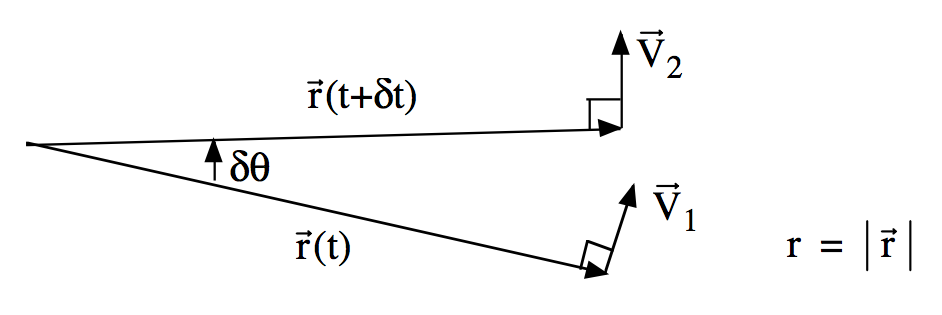
\includegraphics[width=0.8\textwidth]{centrifugal1}	
	\end{figure}
\end{itemize}
\end{frame}
%------------------------------------------------
\begin{frame}{Conservation of Momentum: Apparent Force (Centrifugal)}
\begin{figure}
		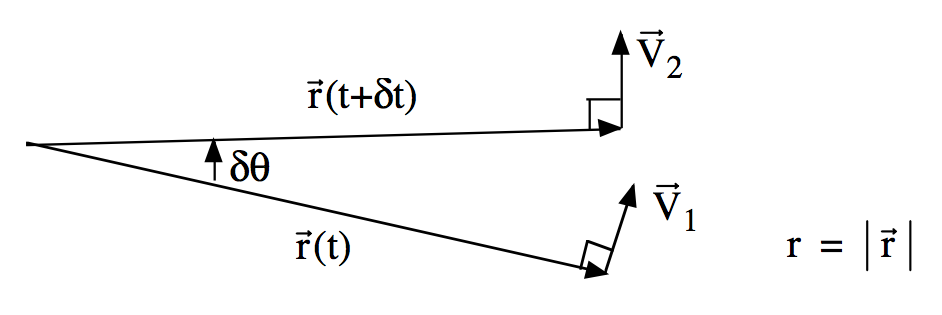
\includegraphics[width=0.8\textwidth]{centrifugal1}	
	\end{figure}
\begin{itemize}
	\item $\omega = d\theta / dt$ $\rightarrow$ thus, the angular displacement $\delta \theta$ of the ball in time $\delta t$ is: $\delta \theta = \omega \delta t$. 
	\item The ball's speed $\left|\vv{V}\right| = \omega r$ is constant since $\omega$, $r$ are constant.
	\item Thus, only the direction of the ball's velocity changes.
\end{itemize}
\end{frame}
%------------------------------------------------
\begin{frame}{Conservation of Momentum: Apparent Force (Centrifugal)}
\begin{figure}
		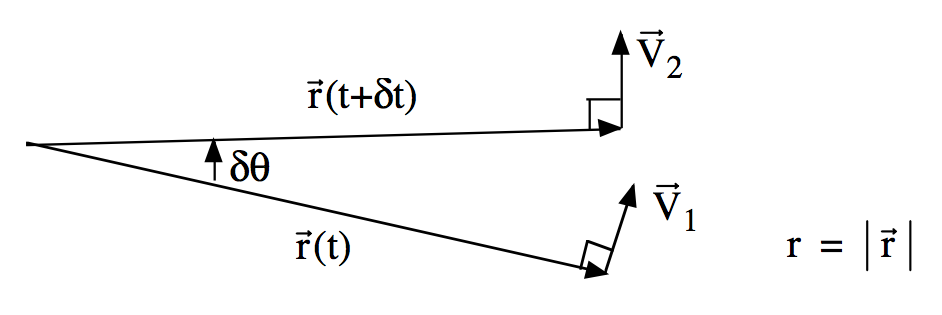
\includegraphics[width=0.8\textwidth]{centrifugal1}	
	\end{figure}
\begin{itemize}
	\item The vector change in $\vv{V}$ over a tiny time increment is $\perp$ to $\vv{V}$.
	\begin{align*}
	\left|\vv{V}\right| &= \text{constant} \rightarrow \sqrt{u^2 + v^2} = \text{constant} \rightarrow u^2 + v^2 = \text{constant}\\
	&\rightarrow \vv{V} \cdot \vv{V} = \text{constant} \rightarrow \frac{D}{Dt}(\vv{V} \cdot \vv{V}) = \frac{D(\text{constant})}{Dt} = 0\\
	&\rightarrow \vv{V}\cdot\frac{D\vv{V}}{Dt} + \vv{V}\cdot\frac{D\vv{V}}{Dt} = 2\vv{V}\cdot\frac{D\vv{V}}{Dt} = 0
	\end{align*}
	Since $\vv{V} \neq 0$ and $\frac{D\vv{V}}{Dt} \neq 0$, must have $\vv{V} \perp \frac{D\vv{V}}{Dt}$
\end{itemize}
\end{frame}
%------------------------------------------------
\begin{frame}{Conservation of Momentum: Apparent Force (Centrifugal)}
\begin{figure}
		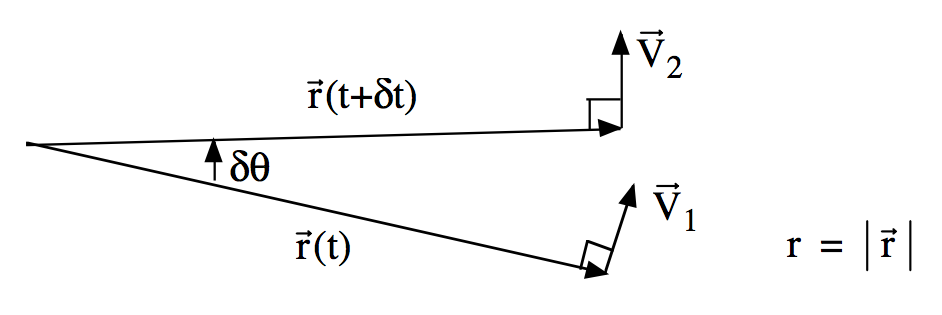
\includegraphics[width=0.8\textwidth]{centrifugal1}	
	\end{figure}
\begin{itemize}
	\item So, the change in $\vv{V}$ (acceleration) is perpendicular to $\vv{V}$
	\item Another way to think about it: there can be no change in $\vv{V}$ in the direction of $\vv{V}$ since $\left|\vv{V}\right|$ is constant. If there was such an acceleration, then $\left|\vv{V}\right|$ would increase/decrease, which is impossible since it is constant. Thus, any change in $\vv{V}$ must be in the radial direction.
\end{itemize}
\end{frame}
%------------------------------------------------
\begin{frame}{Conservation of Momentum: Apparent Force (Centrifugal)}

\begin{itemize}
	\item We can see it graphically
	\begin{figure}
		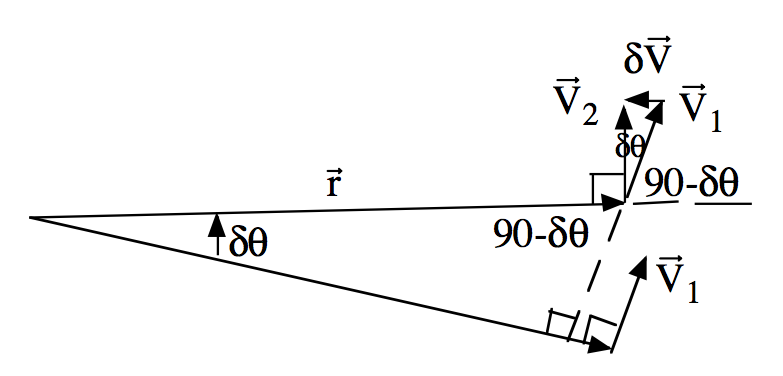
\includegraphics[width=0.7\textwidth]{centrifugal2}	
	\end{figure}
	For small $\delta \theta$, $\delta \vv{V}$ is perpendicular to $\vv{V}$ ($\vv{V_1}$ or $\vv{V_2}$) - meaning it points toward the axis of rotation ($-\hat r$ direction).
\end{itemize}
\end{frame}
%------------------------------------------------
\begin{frame}{Conservation of Momentum: Apparent Force (Centrifugal)}

\begin{itemize}
	\item In the previous example, consider a circle with radius $\left|\vv{V}\right|$
	\begin{figure}
		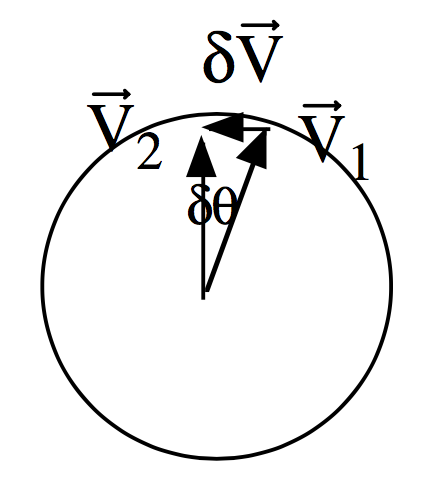
\includegraphics[width=0.2\textwidth]{centrifugal3}	
	\end{figure}
	$$\left|\delta \vv{V}\right| = \left|\vv{V}\right|\delta \theta = -\omega r \delta \theta \rightarrow \delta \vv{V} = -\omega r \delta \theta \hat r$$
	divide bt $\delta t$
	$$\frac{\delta \vv{V}}{\delta t} = -\omega r \frac{\delta \theta}{\delta t} \hat r$$
	Take the limit as $\delta t\rightarrow 0$
	$$\frac{D\vv{V}}{Dt} = -\omega r \frac{D\theta}{Dt} \hat r = -\omega^2 r \hat r = -\omega^2 \vv{r}$$ 
	Thus, the acceleration of the ball is inward toward to the axis of rotation and is called the centripetal acceleration.
\end{itemize}
\end{frame}
%------------------------------------------------
\begin{frame}{Conservation of Momentum: Apparent Force (Centrifugal)}

\begin{itemize}
	\item The force causing this centripetal acceleration is the string pulling inward on the ball:
	\begin{figure}
		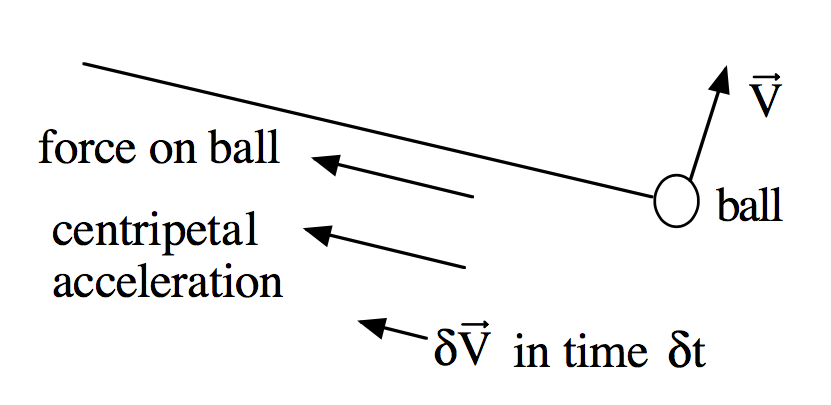
\includegraphics[width=0.8\textwidth]{centrifugal4}	
	\end{figure}
	\item Can apply $\vv{F} = m\vv{a}$ since we are in an inertial reference frame:
	$$\vv{F}_{\text{on ball due to string}} = -m \omega^2 \vv{r}$$
\end{itemize}
\end{frame}
%------------------------------------------------
\begin{frame}{Conservation of Momentum: Apparent Force (Centrifugal)}

\begin{itemize}
	\item Consider the same physical problem, but now our observer (reference frame) is now fixed with respect to the ball.
	\item The ball appears stationary in this non-inertial reference frame, so the apparent acceleration is 0.
	\item However, there is still a force on the ball due to the string!
	\item Applying Newton's \nth{2} Law in this non-inertial reference frame says $\vv{F}_{\text{on ball due to string}} = 0$ which is wrong since a force does exist.
\end{itemize}
\end{frame}
%------------------------------------------------
\begin{frame}{Conservation of Momentum: Apparent Force (Centrifugal)}

\begin{itemize}
	\item To make Newton's \nth{2} Law work in our non-inertial reference frame we need to introduce an ``apparent'' force that cancels with the force on the string.
	\item This apparent force is called the \textbf{centrifugal force}.
	$$\vv{F}_{\text{on ball due to string}} + \vv{F}_{\text{centrifugal}} = 0$$
	thus,
	\begin{align*}
	\vv{F}_{\text{centrifugal}} &= -\vv{F}_{\text{on ball due to string}}\\
	\vv{F}_{\text{centrifugal}} &= m\omega^2\vv{r}
	\end{align*}
\end{itemize}
\end{frame}
%------------------------------------------------
\begin{frame}{Conservation of Momentum: Apparent Force (Centrifugal)}

\begin{itemize}
	\item Instead of a ball, consider a reference frame that is fixed with respect to Earth.
	\item Earth rotates with angular velocity $\vv{\Omega}$ ($\Omega \equiv \left| \vv{\Omega}\right|$)
	\item Consider a mass $m$ at rest on the surface of Earth, $\vv{R}$ is the position vector of this mass with respect to the axis of rotation.
	\item We arrive at the centrifugal force per unit mass:
	$$\boxed{\frac{\vv{F}_{\text{centrifugal}}}{m} = \Omega^2\vv{R}}$$
\end{itemize}
\end{frame}
%------------------------------------------------
\begin{frame}{Conservation of Momentum: Apparent Force (Centrifugal)}

\begin{itemize}
	\item We can now define the \textit{effective gravity}, which is the sum of the fundamental gravitational force and the apparent centrifugal force:
	$$\underbrace{\vv{g}}_{\text{gravity force}} = \underbrace{\vv{g^*}}_{\text{gravitational force}} + \underbrace{\Omega^2 \vv{R}}_{\text{centrifugal force}}$$
	\begin{figure}
		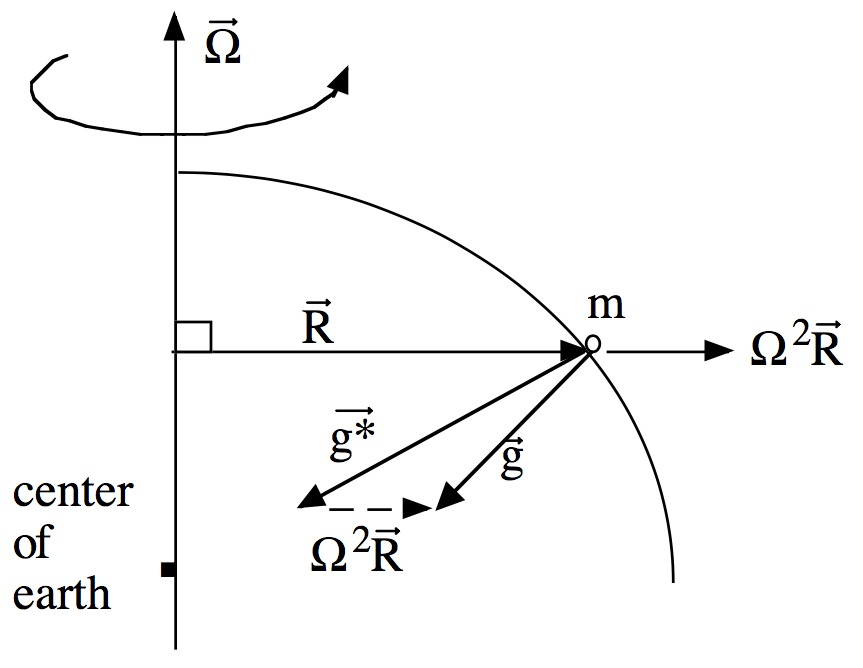
\includegraphics[width=0.6\textwidth]{centrifugal5.png}	
	\end{figure}
\end{itemize}
\end{frame}
%------------------------------------------------
\begin{frame}{Conservation of Momentum: Apparent Force (Coriolis)}

\begin{itemize}
	\item We considered a mass at rest on Earth's surface. 
	\item What happens if the mass is moving?
	\item We will need to introduce a second apparent force to enable the use of Newton's \nth{2} Law.
	\item This apparent force related to movement in the rotating reference frame is named after French scientist Gaspard-Gustave de Coriolis.
\end{itemize}
\end{frame}
%------------------------------------------------
\begin{frame}{Conservation of Momentum: Apparent Force (Coriolis)}

\begin{itemize}
	\item Let's define velocity in terms of Earth
	\begin{figure}
		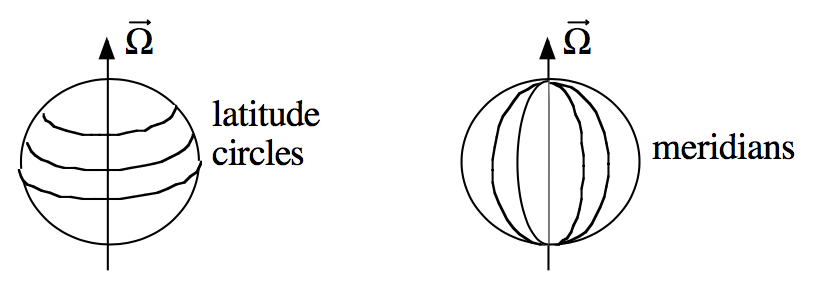
\includegraphics[width=0.5\textwidth]{coriolis1}	
	\end{figure}
	\item $u$ = velocity along a latitude circle
	\begin{itemize}
		\item $u > 0$ toward east (westerly wind)
		\item $u < 0$ toward west (easterly wind)
	\end{itemize}
	\item $v$ = velocity along a meridian
	\begin{itemize}
		\item $v > 0$ toward north (southerly wind)
		\item $v < 0$ toward south (northerly wind)
	\end{itemize}
	\item $w$ = vertical velocity
	\begin{itemize}
		\item $w > 0$ upward motion
		\item $w < 0$ downward motion
	\end{itemize}
\end{itemize}
\end{frame}
%------------------------------------------------
\begin{frame}{Conservation of Momentum: Apparent Force (Coriolis)}

\begin{itemize}
	\item Imagine that we kick an initially resting mass $m$ toward the east.
	\item Since $u>0$ here, the mass rotates faster than earth.
	\item The centrifugal force on the initially resting mass was:
	$$\Omega^2 \vv{R}$$
	\item The centrifugal force on the mass after being kicked:
	$$\left(\Omega + \frac{u}{R}\right)^2 \vv{R}$$
	Note: velocity = angular velocity $\times$ radius, so angular velocity = velocity/radius
\end{itemize}
\end{frame}
%------------------------------------------------
\begin{frame}{Conservation of Momentum: Apparent Force (Coriolis)}

$$\left(\Omega + \frac{u}{R}\right)^2 \vv{R} = \underbrace{\Omega^2\vv{R}}_{\text{centrifugal force}} + \underbrace{2\Omega u \frac{\vv{R}}{R}}_{\text{Coriolis force}} + \underbrace{\frac{u^2}{R^2}\vv{R}}_{\text{small, neglect}}$$
\begin{itemize}
	\item Coriolis force in this scenario is directed radially outward from the axis of rotation. 
	\item Coriolis has no component in latitudinal directions and projects into the meridional and vertical directions.
	\begin{figure}
		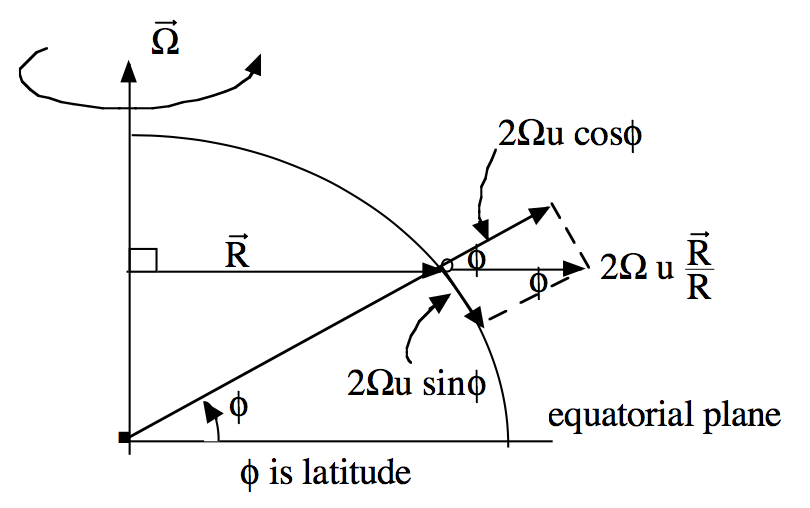
\includegraphics[width=0.6\textwidth]{coriolis2}
	\end{figure}
\end{itemize}
\end{frame}
%------------------------------------------------
\begin{frame}{Conservation of Momentum: Apparent Force (Coriolis)}
\begin{figure}
		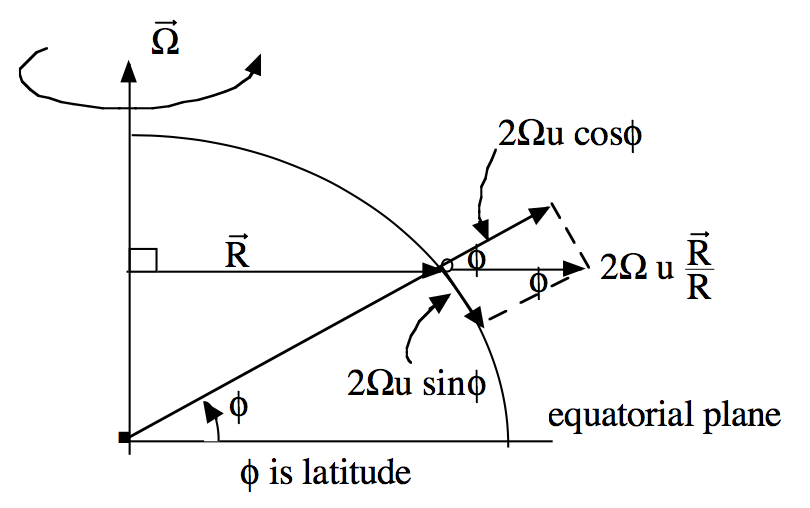
\includegraphics[width=0.6\textwidth]{coriolis2}
	\end{figure}
\begin{itemize}
	\item Associated with this Coriolis force are the following acceleration components:
	$$\left.\frac{dv}{dt}\right|_{\text{Coriolis}} = -2\Omega u \sin \phi \qquad \left.\frac{dw}{dt}\right|_{\text{Coriolis}} = 2\Omega u \cos \phi$$
\end{itemize}
\end{frame}
%------------------------------------------------
\begin{frame}{Conservation of Momentum: Apparent Force (Coriolis)}
$$\left.\frac{dv}{dt}\right|_{\text{Coriolis}} = -2\Omega u \sin \phi \qquad \left.\frac{dw}{dt}\right|_{\text{Coriolis}} = 2\Omega u \cos \phi$$
	\begin{itemize}
	\item $u > 0$ (eastward): acceleration is toward the south and upward (upward Coriolis force is weak compared to gravity and slightly lessens the apparent weight of an object)
	\item $u < 0$ (westward): acceleration is toward the north and downward (slightly increases the apparent weight of an object)
	\item In either case, the Coriolis force is perpendicular to the direction of motion.
	\item In either case, we get a deflection to the left relative to the direction of motion.
\end{itemize}
\end{frame}
%------------------------------------------------
\begin{frame}{Conservation of Momentum: Apparent Force (Coriolis)}

\begin{itemize}
	\item Imagine that we kick an initially resting mass $m$ toward the south ($v<0$)
	\begin{figure}
		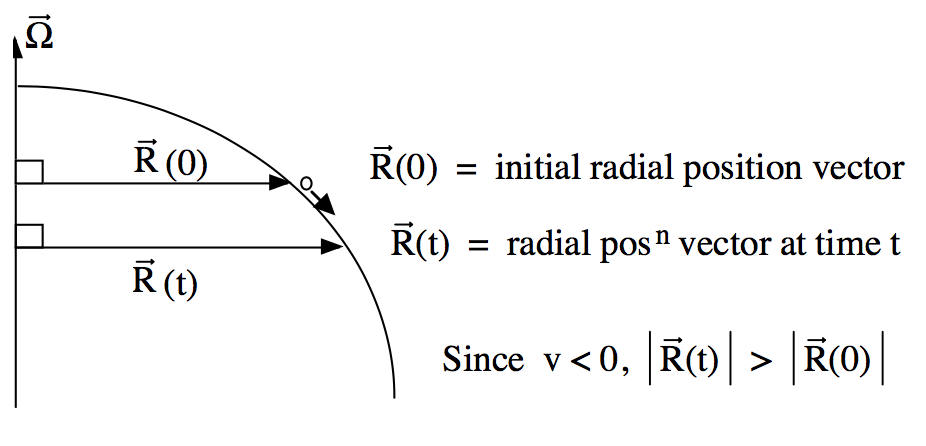
\includegraphics[width=0.7\textwidth]{coriolis3}	
	\end{figure}
	\item From the conservation of angular momentum:
	$$\left[ u(t) + \Omega R(t)\right]R(t) = C$$
	\item Initial conditions will help us solve $C$.
\end{itemize}
\end{frame}
%------------------------------------------------
\begin{frame}{Conservation of Momentum: Apparent Force (Coriolis)}
\begin{figure}
		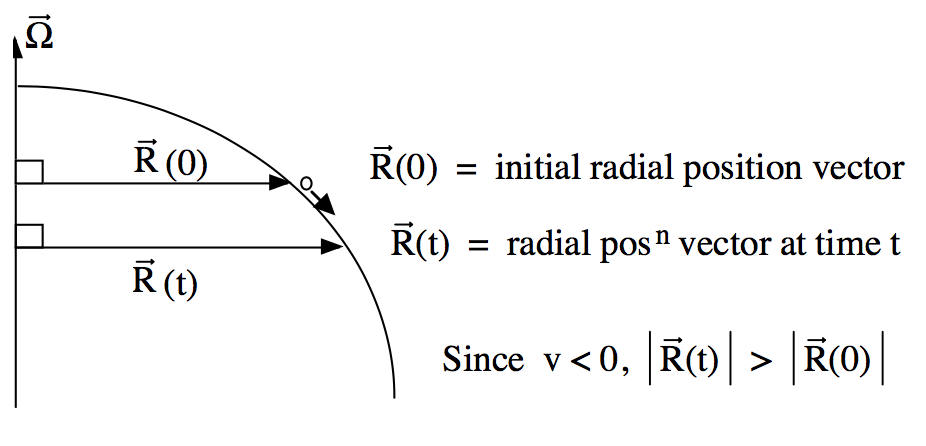
\includegraphics[width=0.7\textwidth]{coriolis3}	
	\end{figure}
\begin{itemize}
	\item At the time of the kick ($t=0$), $u(0) = 0$, and $R = R(0)$:
	$$\left[0 + \Omega R(0)\right]R(0) = C \rightarrow C= \Omega R^2(0)$$
	Thus,
	$$\left[ u(t) + \Omega R(t)\right] R(t) = \Omega R^2(0)$$
\end{itemize}
\end{frame}
%------------------------------------------------
\begin{frame}{Conservation of Momentum: Apparent Force (Coriolis)}

\begin{itemize}
	\item A short time after the kick ($t=\delta t$) the mass is at radius $R(0) + \delta R$ with a southward velocity ($v<0$). $u$? (we will call it $\delta u$ since we expect that it will be small for small $\delta t$
	$$\left\{ \delta u + \Omega \left[ R(0) + \delta R\right]\right\}\left[R(0) + \delta R\right] = \Omega R^2(0)$$
	$$\delta u R(0) + \cancelto{}{\Omega R^2(0)} + \Omega R(0) \delta R + \underbrace{\delta u \delta R}_{\text{small}} + \Omega R(0) \delta R + \underbrace{\Omega(\delta R)^2}_{\text{small}} = \cancelto{}{\Omega R^2(0)}$$ 
	So, we neglect $\delta u \delta R$ and $\Omega(\delta R)^2$
	$$\delta u R(0) + 2\Omega R(0) \delta R = 0 \rightarrow \delta u = -2\Omega \delta R$$
	\item The mass develops a small westward (easterly) velocity component.
	\item Let's describe the acceleration.
\end{itemize}
\end{frame}
%------------------------------------------------
\begin{frame}{Conservation of Momentum: Apparent Force (Coriolis)}
\begin{figure}
		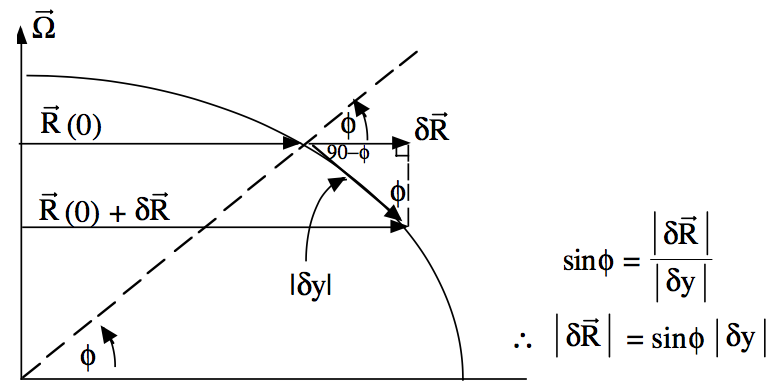
\includegraphics[width=0.6\textwidth]{coriolis4}	
	\end{figure}
\begin{itemize}
	\item $\delta R=-\sin \phi \delta y$ (negative since $\delta y$ corresponds to a postive $\delta R$ (and reverse).
	$$\delta u = - 2\Omega \delta R = -2\Omega (-\sin \phi \delta y) = 2\Omega \sin \phi \delta y$$
	Divide by $\delta t$ and take the limit as $\delta t \rightarrow 0$
	$$\left.\frac{du}{dt}\right|_{\text{Coriolis}} = 2\Omega \sin \phi \frac{dy}{dt} = 2\Omega v \sin \phi$$
\end{itemize}
\end{frame}
%------------------------------------------------
\begin{frame}{Conservation of Momentum: Apparent Force (Coriolis)}
\begin{figure}
		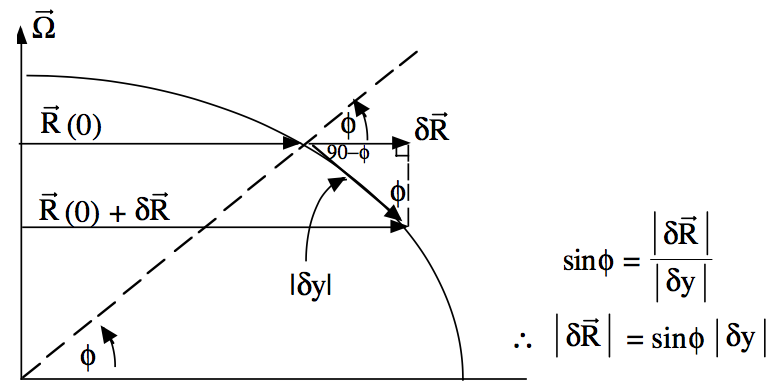
\includegraphics[width=0.6\textwidth]{coriolis4}	
	\end{figure}
\begin{itemize}
	\item For our initial southward kick ($v<0$), $du/dt|_{\text{Coriolis}} < 0$
	\item $u$ is initially $0$ but becomes negative
	\item This means that we get a deflection toward the west (right, relative to the direction of motion)
	\item We get the same formula and rightward deflection if the ball is kicked north.
\end{itemize}
\end{frame}
%------------------------------------------------
\begin{frame}{Conservation of Momentum: Apparent Force (Coriolis)}
\begin{itemize}
	\item Imagine that we kick an initially resting mass $m$ upward ($w>0$) or downward ($w<0$).
	\item Conservation of angular momentum leads to:
	$$\frac{du}{dt}|_{\text{Coriolis}} = -2\Omega w \cos \phi$$
	\item This is derived following a similar approach as for the horizontal components of momentum.
\end{itemize}
\end{frame}
%------------------------------------------------
\begin{frame}{Conservation of Momentum: Apparent Force (Coriolis)}
\begin{itemize}
	\item Putting the all together:
	\begin{align*}
		\frac{du}{dt}|_{\text{Coriolis}} &= 2\Omega v \sin \phi - 2\Omega w \cos \phi\\
		\frac{dv}{dt}|_{\text{Coriolis}} &= -2\Omega u \sin \phi \\
		\frac{dw}{dt}|_{\text{Coriolis}} &= 2\Omega u \cos \phi
	\end{align*}
	\item These terms must appear as apparent forces per unit mass to allow the application of $\vv{F} = m\vv{a}$.
\end{itemize}
\end{frame}
%------------------------------------------------
\end{document}

